\documentclass{beamer}
\usepackage{tfrupee}
\usetheme{Madrid}
\usepackage{amsmath,amssymb,amsfonts,amsthm}
\usepackage{graphicx}
\usepackage{xcolor}
\usepackage{listings}
\usepackage{enumitem}
\usepackage{mathtools}
\usepackage{gensymb}
\usepackage{comment}
\usepackage{hyperref}
\usepackage{multirow}
\usepackage{hhline}

\title{Question-3.4.2.3}
\author{EE24BTECH11048 - NITHIN.K}
\institute{\textbf{LU Decomposition using Doolittle's Algorithm}}
\date{\today}

\begin{document}

\begin{frame}
    \titlepage
\end{frame}

\begin{frame}{Problem Statement}
    \textbf{Question:} The sum of the two digits of a two-digit number is 9. Also, nine times this number is twice the number obtained by reversing the order of the digits.
\end{frame}

\begin{frame}{Mathematical Formulation}
    \begin{align}
        x + y &= 9 \\
        9(10x + y) &= 2(10y + x) \\
        8x - y &= 0
    \end{align}
    The system of equations can be written as:
    \begin{align}
        A\vec{x} = \vec{b}
    \end{align}
    where
    \begin{align}
        A = \begin{bmatrix}1 & 1 \\ 8 & -1\end{bmatrix}, \quad \vec{x} = \begin{bmatrix}x \\ y\end{bmatrix}, \quad \vec{b} = \begin{bmatrix}9 \\ 0\end{bmatrix}
    \end{align}
\end{frame}

\begin{frame}{LU Decomposition - Doolittle's Algorithm}
    The LU decomposition splits $A$ into:
    \begin{align}
        A = LU
    \end{align}
    where \textbf{L} is lower triangular and \textbf{U} is upper triangular:
    \begin{align}
        L = \begin{bmatrix} 1 & 0 \\ L_{21} & 1 \end{bmatrix}, \quad
        U = \begin{bmatrix} U_{11} & U_{12} \\ 0 & U_{22} \end{bmatrix}
    \end{align}
\end{frame}

\begin{frame}{LU Decomposition Computation}
    Elements of \textbf{U}:
    \begin{align}
        U_{ij} = A_{ij} - \sum_{k=0}^{i-1} L_{ik} U_{kj}
    \end{align}
    Elements of \textbf{L}:
    \begin{align}
        L_{ij} = \frac{A_{ij} - \sum_{k=0}^{j-1} L_{ik} U_{kj}}{U_{jj}}
    \end{align}
    Performing LU Decomposition, we get:
    \begin{align}
        L = \begin{bmatrix}1 & 0 \\ 8 & 1\end{bmatrix}, \quad U = \begin{bmatrix}1 & 1 \\ 0 & -9\end{bmatrix}
    \end{align}
\end{frame}

\begin{frame}{Solving the System}
    Forward substitution to solve $L\vec{y} = \vec{b}$:
    \begin{align}
        \begin{bmatrix}1 & 0 \\ 8 & 1\end{bmatrix} \begin{bmatrix}y_1 \\ y_2\end{bmatrix} = \begin{bmatrix}9 \\ 0\end{bmatrix}
    \end{align}
    \begin{align}
        y_1 = 9, \quad y_2 = -72
    \end{align}
    Backward substitution to solve $U\vec{x} = \vec{y}$:
    \begin{align}
        \begin{bmatrix}1 & 1 \\ 0 & -9\end{bmatrix} \begin{bmatrix}x \\ y\end{bmatrix} = \begin{bmatrix}9 \\ -72\end{bmatrix}
    \end{align}
    \begin{align}
        y = 8, \quad x = 1
    \end{align}
\end{frame}

\begin{frame}{Final Answer}
    \textbf{Solution:} The values of $x$ and $y$ are:
    \begin{align}
        x = 1, \quad y = 8
    \end{align}
    \centering
    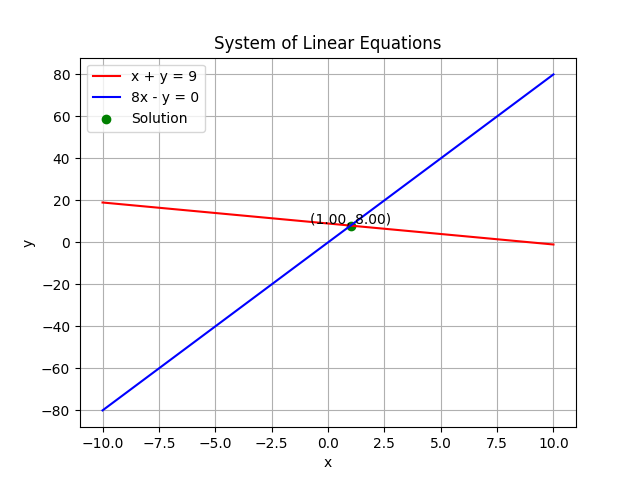
\includegraphics[width=0.8\textwidth]{figs/fig.png}
\end{frame}

\end{document}

